\section{RatioCut谱划分}
\label{sec:graph-ratiocut}

给定一张图，要把顶点分成两个非空组。边的两个端点分在不同组时，需要付出这条边的权重。如果只求割权最小，把一个度最低的顶点单独切出来往往就够了，但这样的分组并不平衡。\term{RatioCut}用两侧的顶点数量调整割权，使得切出很小一组的方案被放大惩罚。

\subsection{RatioCut的谱松弛}
\label{sec:graph-ratiocut-relaxation}

设第一组为$S$，第二组为$\bar S=V\setminus S$，两组的顶点数分别为$s=|S|$和$t=|\bar S|$，满足$s+t=n$。将割权分别除以两组大小，再相加，定义
\begin{equation}
\label{eq:graph-ratiocut}
\operatorname{RatioCut}(S)=c(S,\bar S)\left(\frac{1}{s}+\frac{1}{t}\right).
\end{equation}
若两种切法的割权相同，其中一种只留下很小的一组，那个组对应的倒数$1/s$就会很大，整体代价随之增大。

在四点路径上，切下端点$1$得到一对三的分组，割权为$1$，代价为$1\cdot(1+1/3)=4/3$。切断中间边得到二对二的分组，割权也为$1$，代价为$1\cdot(1/2+1/2)=1$。中间割在RatioCut意义下更优。

目标是在所有非空二分中找出代价最小的分组。为了用拉普拉斯的谱工具求解，我们先把分组编码为一个向量。

给$S$上的顶点赋$1$，$\bar S$上的赋$0$，得到指示向量$\bm 1_S$。跨边的两端相差$1$，组内边的两端相差$0$，因此沿边能量$\bm 1_S^\top\bm L\bm 1_S$恰好等于割权$c(S,\bar S)$。

但这个向量的坐标和为$s$，不满足式~\eqref{eq:graph-algebraic-connectivity}的正交条件$\bm x\perp\bm 1$。将每个坐标减去均值$s/n$，得到
\[
\bm y=\bm 1_S-\frac{s}{n}\bm 1.
\]
$\bm y$在$S$上取$t/n$，在$\bar S$上取$-s/n$。两侧之差仍为$t/n-(-s/n)=1$，跨边的能量不变，组内边仍无贡献。因此$\bm y^\top\bm L\bm y=c(S,\bar S)$。

向量的长度平方按两侧计算：
\[
\bm y^\top\bm y
=s\left(\frac{t}{n}\right)^{\!2}+t\left(\frac{s}{n}\right)^{\!2}
=\frac{st}{n}.
\]
将$\bm y$归一化为$\bm x=\bm y/\|\bm y\|$，它的长度变为$1$，坐标和仍为$0$。能量被除以$\|\bm y\|^2=st/n$，得到
\[
\bm x^\top\bm L\bm x
=\frac{n}{st}\,c(S,\bar S)
=c(S,\bar S)\left(\frac{1}{s}+\frac{1}{t}\right)
=\operatorname{RatioCut}(S).
\]
最后一步用到$n/(st)=1/s+1/t$。这就解释了两组顶点数的倒数之和为什么会出现。

以四点路径的中间割为例，$s=t=2$，归一化后的向量为$(1/2,1/2,-1/2,-1/2)^\top$。唯一的非零边差等于$1$，能量为$1$，恰好等于这个割的RatioCut值。

到此为止，向量$\bm x$只能取由分组确定的两个值。这个离散限制使得问题在组合意义上是困难的。谱松弛去掉两值限制，只保留$\bm x\perp\bm 1$和$\|\bm x\|=1$这两个条件。松弛后的最小值就是组合拉普拉斯的第二小特征值$\lambda_2$。

原来的每个分组向量都满足这两个条件，因而$\lambda_2$不超过任何实际RatioCut值。它是离散最优值的一个下界。

图~\ref{fig:graph-ratiocut-relaxation}对比了实际分组和松弛解。中间割的两值向量只在一条边上有变化，所有能量集中在那里。松弛解允许数值在多条边上逐步过渡，沿边能量因此更小。

\begin{BookInlineFigure}
  \centering
  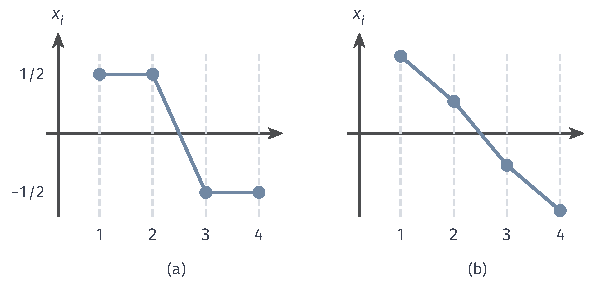
\includegraphics{figures/03-graphs/05-matrices-and-spectra/tikz/ratiocut-relaxation/figure.pdf}
  \caption{单位权四点路径的两种赋值。横轴按路径顺序标出顶点，纵轴是赋值。(a) 中间割的两值向量，能量为$1$。(b) 松弛后得到的第二特征向量，能量为$2-\sqrt2$。两者的坐标和都为零，长度都为一。}
  \label{fig:graph-ratiocut-relaxation}
\end{BookInlineFigure}

松弛给出了下界和一个连续方向，但这个方向本身不是合法的分组。下一步要把实数值的特征向量转换成可以在原图中使用的两组顶点。

\subsection{算法实现}
\label{sec:graph-ratiocut-sweep}

思路是按特征向量的分量从大到小排序，在相邻不同值之间逐个试切，并为每个候选分组计算原始的RatioCut目标。

\begin{algorithm}[RatioCut阈值扫描]
\label{alg:graph-ratiocut-sweep}
给定有限非负加权图，输出非空二分及其RatioCut值。
\begin{enumerate}
\item 若图不连通，选一个连通分量为一侧，另一侧为其余顶点。两侧之间没有正权边，割权为零，返回零代价的分组。
\item 否则求组合拉普拉斯的第二特征向量。按分量从大到小排序。分量相同的顶点作为一组，不能拆开。
\item 从空集开始逐组加入顶点。加入时更新割权：从当前割权中减去新顶点连向已选顶点的边权（这些边从跨边变为组内边），加上连向仍未入选顶点的边权（这些边从组内边变为跨边）。
\item 每组加入后，若两侧均非空，按式~\eqref{eq:graph-ratiocut}计算RatioCut。比较所有候选，返回目标值最小的分组。
\end{enumerate}
\end{algorithm}

\paragraph{执行过程}

在单位权四点路径上，第二特征向量可取为
\[
\bm x=(a,b,-b,-a)^\top,
\qquad a=\cos(\pi/8),\quad b=\cos(3\pi/8).
\]
因为$a>b>0$，顶点按$1,2,3,4$的顺序入选。

第一步放入顶点$1$。它只有一条边连向尚未入选的顶点$2$，割权变为$1$。第二步放入$2$时，边$12$从跨边变成组内边（割权减$1$），但边$23$从组内变为跨边（割权加$1$），割权仍为$1$。第三步放入$3$时，类似地跨边改成$34$。

三个候选的计算如下。
\begin{center}
\begin{tabular}{lccc}
\toprule
已选集合 & 两侧大小 & 割权 & RatioCut\\
\midrule
$\{1\}$ & $1,3$ & $1$ & $4/3$\\
$\{1,2\}$ & $2,2$ & $1$ & $1$\\
$\{1,2,3\}$ & $3,1$ & $1$ & $4/3$\\
\bottomrule
\end{tabular}
\end{center}

图~\ref{fig:ratiocut-sweep-candidates}按排序顺序画出四个顶点，并标出三种切分位置。每条竖线对应一种候选，线两侧的集合、割边及RatioCut值都标在旁边。观察中间切法如何同时使两侧大小均匀且割权不增。

\begin{figure}[!htb]
\centering
\begin{tikzpicture}[x=1mm,y=1mm,>=Stealth,
  vertex/.style={circle,draw=FigureBlue,fill=FigureBlueFill,inner sep=0pt,
    minimum size=5mm,line width=.52pt,font=\figurefont\fontsize{8}{10}\selectfont},
  cutline/.style={dashed,FigureRed,line width=.6pt},
  clabel/.style={font=\figurefont\fontsize{7}{8.5}\selectfont,FigureRed},
  vlabel/.style={font=\figurefont\fontsize{7.5}{9}\selectfont,FigureInk}]
  % vertices on a line
  \node[vertex] (v1) at (0,0) {$1$};
  \node[vertex] (v2) at (16,0) {$2$};
  \node[vertex] (v3) at (32,0) {$3$};
  \node[vertex] (v4) at (48,0) {$4$};
  \draw[FigureStroke,line width=.52pt] (v1)--(v2)--(v3)--(v4);
  % Cut 1: after vertex 1
  \draw[cutline] (8,7) -- (8,-7);
  \node[clabel,above] at (8,7.5) {$\frac{4}{3}$};
  % Cut 2: after vertex 2
  \draw[cutline] (24,7) -- (24,-7);
  \node[clabel,above] at (24,7.5) {$1$};
  % Cut 3: after vertex 3
  \draw[cutline] (40,7) -- (40,-7);
  \node[clabel,above] at (40,7.5) {$\frac{4}{3}$};
  % vertex ordering label
  \node[vlabel] at (24,-12) {按特征向量分量从大到小排序};
\end{tikzpicture}
\caption{四点路径上的RatioCut阈值扫描。四个顶点按第二特征向量分量递减排列。红色虚线标出三种切分位置，上方数字是对应的RatioCut值。中间割的代价最低。}
\label{fig:ratiocut-sweep-candidates}
\end{figure}

中间割的代价最小，为$1$。这是扫描得到的实际分组代价，可以和松弛下界$\lambda_2=2-\sqrt2\approx0.586$放在一起比较。

\subsection{算法分析}
\label{sec:graph-ratiocut-guarantee}

记所有非空二分中的RatioCut最小值为$\operatorname{OPT}_R$，扫描返回的分组为$S_R$。松弛扩大了可行域，给出下界；扫描提供了一个具体的可行割，给出上界：
\begin{equation}
\label{eq:graph-ratiocut-bounds}
\lambda_2\leq\operatorname{OPT}_R
\leq\operatorname{RatioCut}(S_R).
\end{equation}

四点路径上可以直接验证$\operatorname{OPT}_R=1$。任何非空二分至少切过一条边（路径是连通的），且两侧顶点数之积$st$至多为$\lfloor n/2\rfloor\cdot\lceil n/2\rceil=4$。因此$1/s+1/t=n/(st)\geq 4/4=1$，任何割的RatioCut都不低于$1$。中间割恰好达到了这个值。

排序$n$个顶点需要$O(n\log n)$时间。扫描过程中每个顶点加入一次，加入时检查它的邻接表，因此所有边在两个端点各被访问至多一次，扫描耗时$O(n+m)$。求特征向量的代价另行计算，取决于所用的迭代方法和精度要求。

一次扫描只比较沿一个排序方向切开的嵌套集合，没有覆盖全部$2^{n-1}-1$个无序二分。选择不同的最优方向（当$\lambda_2$为重根时）或近似方向可能给出不同的候选。相同分量作为一组处理，减少了切点数量。

精确的$\lambda_2$是有效的下界。但如果使用的是数值迭代得到的近似特征向量，代入Rayleigh商所得的值大于或等于$\lambda_2$，不一定仍是离散最优值的下界。报告结果时应区分：认证过误差的下界和数值估计值。扫描得到的分组及其原目标代价可以直接在原图上核对，不受特征向量精度的影响。
